\documentclass{article}
\usepackage[T1]{fontenc}
\usepackage[utf8]{inputenc}
\usepackage{amsmath,amssymb,amsfonts}
\usepackage[english,main=russian]{babel}
\usepackage{graphicx}
\graphicspath{{.}}
\newcommand\xp{\frac{21+\sqrt{385}}{14}}
\newcommand\xn{\frac{21-\sqrt{385}}{14}}

\begin{document}
\textbf{1. Какова вероятность того, что сумма двух наугад взятых положительных чисел, каждое из которых не больше трех, не превзойдет трех, а их произведение будет не больше 2/7?}

Пусть $x, y$ - два выбранных числа. Имеем следующую систему:

$\begin{cases}
    0 \leq x \leq 3 & \quad (1) \\
    0 \leq y \leq 3 & \quad(2)\\
    x + y \leq 3 & \quad(3)\\
    x * y \leq \frac{2}{7} & \quad (4)
\end{cases}$

Найдем нужную вероятность как геометрическую: мера пространства элементарных исходов равна 9, мера события - площадь, выделенная на графике:

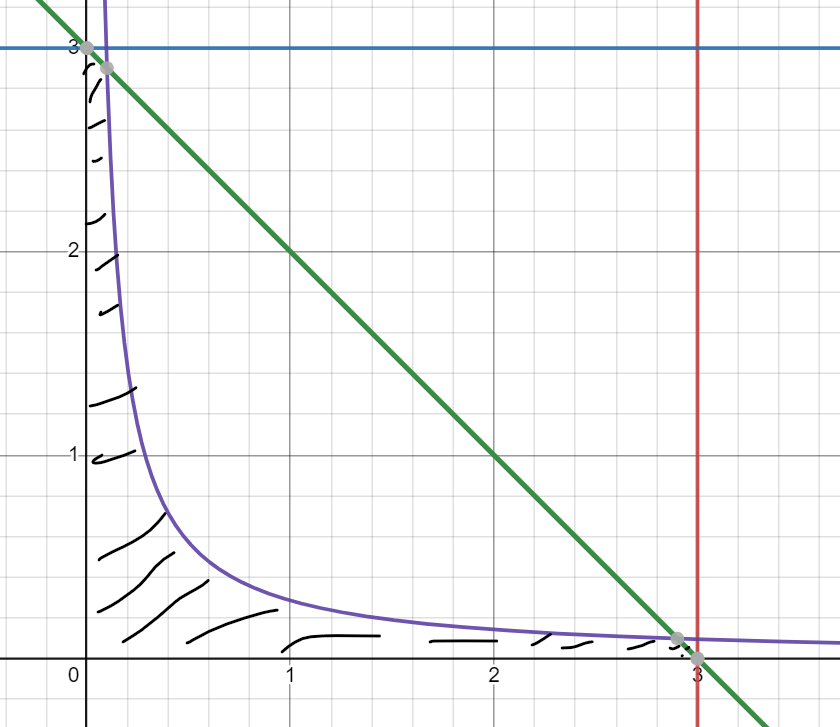
\includegraphics[width=100mm]{graph}

Посчитаем выделенную площадь(назовем её S) как сумму: 2 треугольников с вершинами $(0,3),(\xn,\xp),(0,\xp)$ и $(3,0),(\xp,\xn),(\xp,0)$, прямоугольник с вершинами $(0,0)(0,\xp)(\xn,\xp) \text{ и }(\xn,0)$ и площадь под гиперболой в точках пересечения уравнений (3) и (4) $\int^{\xp}_{\xn}(\frac{2}{7x})dx$

Тогда $S = 2 * \frac{59-3*\sqrt{385}}{14} + \frac{2}{7} + \frac{2}{7} * \ln({\frac{59+3\sqrt{385}}{4})}$

В ответе $P = \frac{S}{9} = \frac{61 - 3\sqrt{385} + 2\ln({\frac{59 + 3\sqrt{385}}{4}})}{63} \approx 0.141305$

\textbf{2. В пассажирском поезде 9 вагонов. Сколькими способами можно рассадить в поезде 4 человека, при условии, что все они должны ехать в различных вагонах?}

Ответ на данную задачу - в точности число размещений - $A^{4}_{9} = \frac{9!}{(9 - 4)!} = 3024$.
Существует 3024 таких способов.

\textbf{3. Для участия в команде тренер отбирает 5 мальчиков из 10. Сколькими способами он может сформировать команду, если 2 определенных мальчика должны войти в команду?}

Так как 2 мальчика в любом случае попадут в команду, т.е. в команде уже есть 2 человека, тренеру необходимо отобрать 3 мальчика из 8 пока что неопредленных. Это  в точности число размещений $A^{3}_{8} = \frac{8!}{(8 - 3)!} = 336$.
Существует 336 таких способов.

\textbf{4. В программе к экзамену по теории вероятностей 75 вопросов. Студент знает 50 из них. В билете 3 вопроса. Найдите вероятность того, что студент знает хотя бы два вопроса из вытянутого им билета.}

Необходимо рассмотреть два случая:
\begin{enumerate}
\item Вероятность выпадение билета, в котором студент знает все вопросы. Как только студент понимает, к какому множеству(выученные, невыученные) относится вопрос, из соответсвующего множества и множества всех вопросов удаляется данный вопрос, если предполагать, что вопросы не повторяются. Поэтому вероятность на выпадение нужного билета будет такой: $\frac{50}{75}*\frac{49}{74}*\frac{48}{73}$;
\item Вероятность выпадение билета, в котором студент знает 2 вопроса. Опираясь на предсатвленные выше рассуждения, можно заключить, что необходимая вероятность будет следующая: $\frac{50}{75}*\frac{49}{74}*\frac{25}{73}$ или $\frac{50}{75}*\frac{25}{74}*\frac{49}{73}$ или $\frac{25}{75}*\frac{50}{74}*\frac{49}{73}$, т.е. $3*\frac{50}{75}*\frac{49}{74}*\frac{25}{73}$.
\end{enumerate}

Вероятность того, что студент знает хотя бы два вопроса из вытянутого им билета, есть сумма вероятностей из двух, вышепредставленных случаев, т.е.
Ответ: $\frac{2009}{2701}$

\textbf{5. Вероятность увидеть машину на трассе за 30 минут — 0.95. Какая вероятность увидеть машину на трассе за 10 мин? }

\textbf{6. Порядок выступления 7 участников конкурса определяется жребием. Сколько различных вариантов жеребьевки при этом возможно?}

Ответ на данную задачу - в точности число перестановок участников конкурса в некотором конкурсном списке, полученном в результате жеребьевки: $P_{7} = 7! = 5040$.
Существует 5040 таких вариантов.
\end{document}